%\documentclass[table, 10pt]{beamer}%
\documentclass[table, 10 pt, handout]{beamer}%

\usepackage[french]{babel}
\usepackage{tikz}
\usepackage[latin1]{inputenc}
\usepackage{times}
\usepackage[T1]{fontenc}

\usepackage{graphicx,graphics}

\usepackage{amsmath,amsfonts}

\usepackage{multirow}

%\usepackage[table]{xcolor}

%\usepackage{beamerthemeliris}

\usepackage{beamerthemesplit}
\usetheme{Malmoe}%Copenhagen%Dresden%Malmoe
\usecolortheme{orchid}%beetle,seagull,crane,dove,orchid
\useinnertheme[shadow]{rounded}%rounded
\usefonttheme{professionalfonts}

\definecolor{darkgreen}{RGB}{0,180,0} 

\setbeamertemplate{navigation symbols}{}


\newenvironment{codeblock}[1]{\begin{exampleblock}<+->{\texttt{#1}}\begin{tt}}{\end{tt}\end{exampleblock}}




\title[S21 - Comprendre les r�seaux -- CM3 - Perl, \hspace{1cm}\insertframenumber{} / \inserttotalframenumber]
{S21 -- Comprendre les r�seaux }
\subtitle{CM3 -- On vous a menti : diff�rence Perl/C}
\author[Julien Gossa]{Julien Gossa}
\institute
{ 
	{\bf IUT Robert Schuman -- D�partement Informatique}\\
	{\url{julien.gossa@urs.u-strasbg.fr}}
}

\date{2009}
\beamertemplatetransparentcovereddynamicmedium 

\begin{document}


\begin{frame}
 	\titlepage
\end{frame}



\AtBeginSection[]
{
   \begin{frame}
       \frametitle{Sans transition\ldots}
       %\small
       \tableofcontents[currentsubsection]
   \end{frame}
}	

\AtBeginSubsection[]
{
   \begin{frame}
       \frametitle{Sans transition\ldots}
       %\small
       \tableofcontents[currentsubsection]
   \end{frame}
}	

\def\imgheight{0.4\textheight}



% ----------------------------------------------------------------------
\begin{frame}

	\begin{block}<+-> {R�seau}
		\begin{itemize}
		\item Complexe
		\item De nombreux param�tres
		\item De nombreuses op�rations
		\end{itemize}	
	\end{block}
	
	\begin{exampleblock}<+-> {Perl}	
		\begin{itemize}
		\item D�veloppement rapide
		\item Param�tres g�r�s automatiquement
		\item Op�rations masqu�es
		\end{itemize}
	\end{exampleblock}
	
	\begin{alertblock}<+-> {C}
		\begin{itemize}
		\item D�veloppement pr�cis
		\item Aucun param�tre g�r� automatiquement
		\item Aucune op�ration masqu�e
		\end{itemize}
	\end{alertblock}		
	
	
\end{frame}
% ----------------------------------------------------------------------


% ----------------------------------------------------------------------
\section{Perl vs C : UDP}
% ----------------------------------------------------------------------

% ----------------------------------------------------------------------
\begin{frame}
	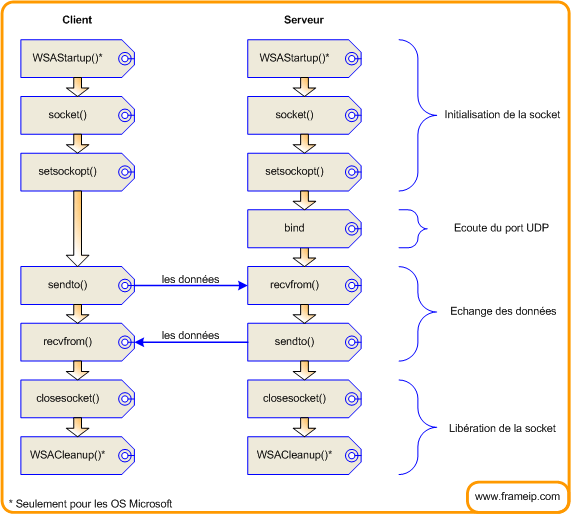
\includegraphics[height=\textheight]{res/c_mode_non_connecte}
\end{frame}
% ----------------------------------------------------------------------

% ----------------------------------------------------------------------
\subsection{Initialisation}
% ----------------------------------------------------------------------
\begin{frame}[fragile]{Initialisation Serveur}

\scriptsize

	\begin{exampleblock}<+-> {Perl}
		\begin{verbatim}
$socket= IO::Socket::INET->new (
  LocalPort => 1234,
  Proto    => "UDP",
  )or die "Impossible d'ouvrir la socket\n";
		\end{verbatim}	
	\end{exampleblock}
	
	
	\begin{alertblock}<+-> {C}
		\begin{verbatim}
id_de_la_socket=socket(AF_INET,SOCK_DGRAM,0);
if (id_de_la_socket==INVALID_SOCKET)
      printf("Impossible d'ouvrir la socket : %d",WSAGetLastError());
      
info_source.sin_family=AF_INET;
info_source.sin_addr.s_addr=INADDR_ANY; // Toutes les IP locales 
info_source.sin_port=htons(1234);       // Port
erreur=bind(
  id_de_la_socket,
  (struct sockaddr*)&information_sur_la_source,
  sizeof(info_source));
if (erreur!=0)
      printf("Impossible d'ecouter le port : %d %d",erreur,WSAGetLastError());
		\end{verbatim}
		
	\end{alertblock}
	
\end{frame}
% ----------------------------------------------------------------------


% ----------------------------------------------------------------------
\begin{frame}[fragile]{Initialisation Client}

\scriptsize

	\begin{exampleblock}<+-> {Perl}
		\begin{verbatim}
$socket= IO::Socket::INET->new (
 	PeerPort => 1234,
 	PeerAddr => "10.0.0.1",
  Proto    => "UDP",
  )or die "Impossible d'ouvrir la socket\n";		
		\end{verbatim}	
	\end{exampleblock}
	
	
	\begin{alertblock}<+-> {C}
		\begin{verbatim}
id_de_la_socket=socket(AF_INET,SOCK_DGRAM,0);
if (id_de_la_socket==INVALID_SOCKET)
      printf("Impossible d'ouvrir la socket : %d",WSAGetLastError());
 		\end{verbatim}
		
	\end{alertblock}
	
\end{frame}
% ----------------------------------------------------------------------


% ----------------------------------------------------------------------
\subsection{\'Echange des donn�es}
% ----------------------------------------------------------------------
\begin{frame}[fragile]{Envoie des donn�es}

\scriptsize

	\begin{exampleblock}<+-> {Perl}
		\begin{verbatim}  
$socket->send($buffer);
		\end{verbatim}	
	\end{exampleblock}
	
	
	\begin{alertblock}<+-> {C}
		\begin{verbatim}		
		
info_destination.sin_family=AF_INET;                     // IPV4
info_destination.sin_port=htons(1234);                   // Port dest
info_destination.sin_addr.s_addr=inet_addr("10.0.0.1");  // IP serveur

nb_caractere=sendto(
  id_de_la_socket,
  buffer,
  strlen(buffer),
  0,
  (struct sockaddr*)&information_sur_la_destination,
  sizeof(info_destination));
  
if (nb_caractere==SOCKET_ERROR)
      printf("Erreur envoie donn�es : %d",WSAGetLastError());		
		\end{verbatim}
		
	\end{alertblock}
	
\end{frame}
% ----------------------------------------------------------------------



% ----------------------------------------------------------------------
\begin{frame}[fragile]{R�ception des donn�es}

\scriptsize

	\begin{exampleblock}<+-> {Perl}
		\begin{verbatim}
$socket->recv($buffer,128);
		\end{verbatim}	
	\end{exampleblock}
	
	
	\begin{alertblock}<+-> {C}
		\begin{verbatim}
tempo=sizeof(information_sur_la_source); 

nb_caractere=recvfrom(
  id_de_la_socket,
  buffer,
  1515,
  0,
  (struct sockaddr*)&information_sur_la_source,
  &tempo);
  
buffer[nb_caractere]=0;                 // Ferme le tableau
		\end{verbatim}
	\end{alertblock}
	
\end{frame}
% ----------------------------------------------------------------------

% ----------------------------------------------------------------------
\subsection{Fermeture}
% ----------------------------------------------------------------------
\begin{frame}[fragile]{Fermeture}

\scriptsize

	\begin{exampleblock}<+-> {Perl}
		\begin{verbatim}
$socket->close() 
or die "Erreur";
		\end{verbatim}	
	\end{exampleblock}
	
	
	\begin{alertblock}<+-> {C}
		\begin{verbatim}
erreur=closesocket(id_de_la_socket);
if (erreur!=0)
      printf("Erreur : %d %d",erreur,WSAGetLastError())
   	\end{verbatim}
	\end{alertblock}
	
\end{frame}
% ----------------------------------------------------------------------


% ----------------------------------------------------------------------
\begin{frame}{Comparaison}

\scriptsize

	\begin{exampleblock}<+-> {Perl vs C}
		\begin{itemize}
		
		\item D�finition automatique du param�tre
			\begin{itemize}
			\item Port local du client
			\item information socket distante
			\end{itemize}	
			
		\item Op�rations automatiques
			\begin{itemize}
			\item send / sendto
			\item recv / recvfrom
			\end{itemize}	
		\end{itemize}			
	\end{exampleblock}
	
		
\end{frame}
% ----------------------------------------------------------------------




% ----------------------------------------------------------------------
\section{Perl vs C : TCP}
% ----------------------------------------------------------------------

% ----------------------------------------------------------------------
\begin{frame}
	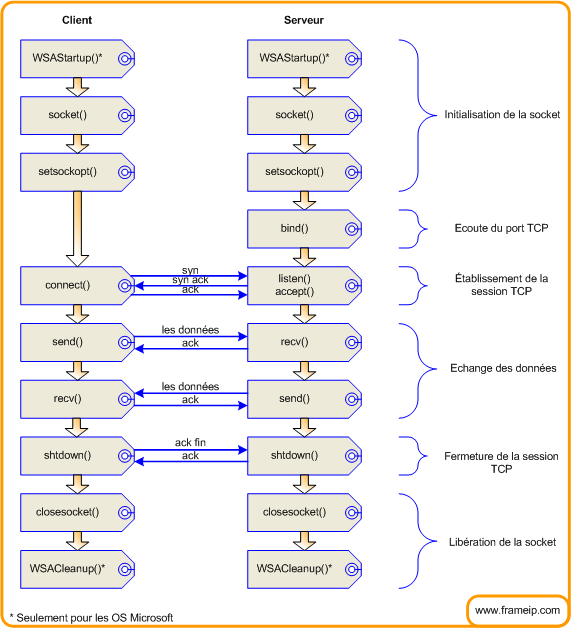
\includegraphics[height=\textheight]{res/c_mode_connecte}
\end{frame}
% ----------------------------------------------------------------------

% ----------------------------------------------------------------------
\subsection{Initialisation}
% ----------------------------------------------------------------------
\begin{frame}[fragile]{Initialisation Serveur}

\scriptsize

	\begin{exampleblock}<+-> {Perl}
		\begin{verbatim}
$socketlisten= IO::Socket::INET->new (
 	PeerPort => 1234,
 	PeerAddr => "10.0.0.1",
  Proto    => "TCP",
  )or die "Impossible d'ouvrir la socket\n";		
 		\end{verbatim}	
	\end{exampleblock}
	
	
	\begin{alertblock}<+-> {C}
		\begin{verbatim}
id_socket_listen=socket(AF_INET,SOCK_STREAM,0);

erreur=setsockopt(id_socket, IPPROTO_TCP, TCP_NODELAY, 
	(char *)&tempo, sizeof(tempo));

erreur=bind( id_de_la_socket,
  (struct sockaddr*)&info_source,
  sizeof(info_source));

info_destination.sin_family=AF_INET;
info_destination.sin_addr.s_addr=inet_addr("10.0.0.1"); // IP serveur
info_destination.sin_port=htons(1234);                  // Port 
erreur=connect( id_socket_listen,
  (struct sockaddr*)&info_destination,
  sizeof(information_sur_la_destination));      
		\end{verbatim}
		
	\end{alertblock}
	
\end{frame}
% ----------------------------------------------------------------------

% ----------------------------------------------------------------------
\begin{frame}[fragile]{Initialisation Client}

\scriptsize

	\begin{exampleblock}<+-> {Perl}
		\begin{verbatim}
$socket= IO::Socket::INET->new (
 	PeerPort => 1234,
 	PeerAddr => "10.0.0.1",
  Proto    => "TCP",
  )or die "Impossible d'ouvrir la socket\n";		
 		\end{verbatim}	
	\end{exampleblock}
	
	
	\begin{alertblock}<+-> {C}
		\begin{verbatim}
id_de_la_socket=socket(AF_INET,SOCK_STREAM,0);
if (id_de_la_socket==INVALID_SOCKET)
      printf("\nDesole, je ne peux pas creer la socket du a l'erreur : %d",WSAGetLastError());
else
      printf("\nsocket      : OK");
      
info_source.sin_family=AF_INET;
info_source.sin_addr.s_addr=INADDR_ANY; // Ecoute sur toutes les IP locales 
info_source.sin_port=htons(33333); // Ecoute sur le port 33333
erreur=bind(id_de_la_socket,(struct sockaddr*)&information_sur_la_source,sizeof(information_sur_la_source));
if (erreur!=0)
      printf("\nDesole, je ne peux pas ecouter ce port : %d %d",erreur,WSAGetLastError());
else
      printf("\nbind        : OK");            
 		\end{verbatim}
		
	\end{alertblock}
	
\end{frame}
% ----------------------------------------------------------------------


% ----------------------------------------------------------------------
\begin{frame}[fragile]{Connexion Serveur}

\scriptsize

	\begin{exampleblock}<+-> {Perl}
		\begin{verbatim}
$socket=socketlisten->accept();
 		\end{verbatim}	
	\end{exampleblock}
	
	
	\begin{alertblock}<+-> {C}
		\begin{verbatim}
while(erreur!=0) 
      erreur=listen(id_de_la_socket,1);
      
tempo=sizeof(info_source);
id_socket=accept(
  id_de_la_socket,
  (struct sockaddr*)&info_source,
  &tempo);
		\end{verbatim}
		
	\end{alertblock}
	
\end{frame}
% ----------------------------------------------------------------------


% ----------------------------------------------------------------------
\begin{frame}[fragile]{Connexion Client}

\scriptsize

	\begin{exampleblock}<+-> {Perl}
Automatique
	\end{exampleblock}
	
	
	\begin{alertblock}<+-> {C}
		\begin{verbatim}
while(erreur!=0) 
      erreur=listen(id_de_la_socket,1);
      
tempo=sizeof(info_source);
id_socket=accept(
  id_de_la_socket,
  (struct sockaddr*)&info_source,
  &tempo);
		\end{verbatim}
		
	\end{alertblock}
	
\end{frame}
% ----------------------------------------------------------------------

% ----------------------------------------------------------------------
\subsection{\'Echange des donn�es}
% ----------------------------------------------------------------------
\begin{frame}[fragile]{Envoie/Reception des donn�es}

\scriptsize

	\begin{exampleblock}<+-> {Perl}
		\begin{verbatim}
$socket->send($buffer);
$socket->recv($buffer,128);
		\end{verbatim}	
	\end{exampleblock}
	
	
	\begin{alertblock}<+-> {C}
		\begin{verbatim}
send(id_socket, buffer, strlen(buffer), 0);
recv(id_socket, buffer, 128, 0);
		\end{verbatim}
		
	\end{alertblock}
	
\end{frame}
% ----------------------------------------------------------------------


% ----------------------------------------------------------------------
\subsection{Fermeture}
% ----------------------------------------------------------------------
\begin{frame}[fragile]{Fermeture}

\scriptsize

	\begin{exampleblock}<+-> {Perl}
		\begin{verbatim}
$socket->close() 
or die "Erreur";
		\end{verbatim}	
	\end{exampleblock}
	
	
	\begin{alertblock}<+-> {C}
		\begin{verbatim}
erreur=closesocket(id_de_la_socket);
if (erreur!=0)
      printf("Erreur : %d %d",erreur,WSAGetLastError())
   	\end{verbatim}
	\end{alertblock}
	
\end{frame}
% ----------------------------------------------------------------------



% ----------------------------------------------------------------------
\section{Perl vs C : Conclusion}
% ----------------------------------------------------------------------

% ----------------------------------------------------------------------
\begin{frame}{Comparaison}

\scriptsize

	\begin{exampleblock}<+-> {Perl vs C}
		\begin{itemize}
		
		\item D�finition automatique
			\begin{itemize}
			\item Port local du client
			\item Et bien d'autres\ldots
			\end{itemize}	
			
		\item Op�rations automatiques
			\begin{itemize}
			\item bind
			\item listen
			\item accept
			\end{itemize}			
		
		\item Format des donn�es
			\begin{itemize}
			\item C : binaire
			\item Perl : scalaire (cha�ne de caract�res)
			\end{itemize}	
			
		\end{itemize}
	\end{exampleblock}
	
\end{frame}
% ----------------------------------------------------------------------

\end{document}